%%%%%%%%%%%%%%%%%%%%%%%%%%%%%%%%%%%%%%%%%%%%%%%%%%%%%%%%%%%%%%%%%%%%
% Overivew
%%%%%%%%%%%%%%%%%%%%%%%%%%%%%%%%%%%%%%%%%%%%%%%%%%%%%%%%%%%%%%%%%%%%


\section{Results and Discussion}
\label{sec:results}

In this section we show how our framework can be used for designing various kinds of interlocking assemblies, with example applications as puzzles, furniture, sculptures, or architectural designs. We highlight differences to previous approaches to show how our method improves the state of the art and enables new kinds of interlocking assemblies not possible before. For more detailed comparisons and results we refer to the supplementary material.

%%%%%%%%%%%%%%%%%%%%%%%%%%%%%%%%%%%%%%%%%%%%%%%%
% 1. Interlocking Puzzle
%%%%%%%%%%%%%%%%%%%%%%%%%%%%%%%%%%%%%%%%%%%%%%%%

\begin{figure*}[!t]
	\centering
	%\vspace*{-3.5mm}
	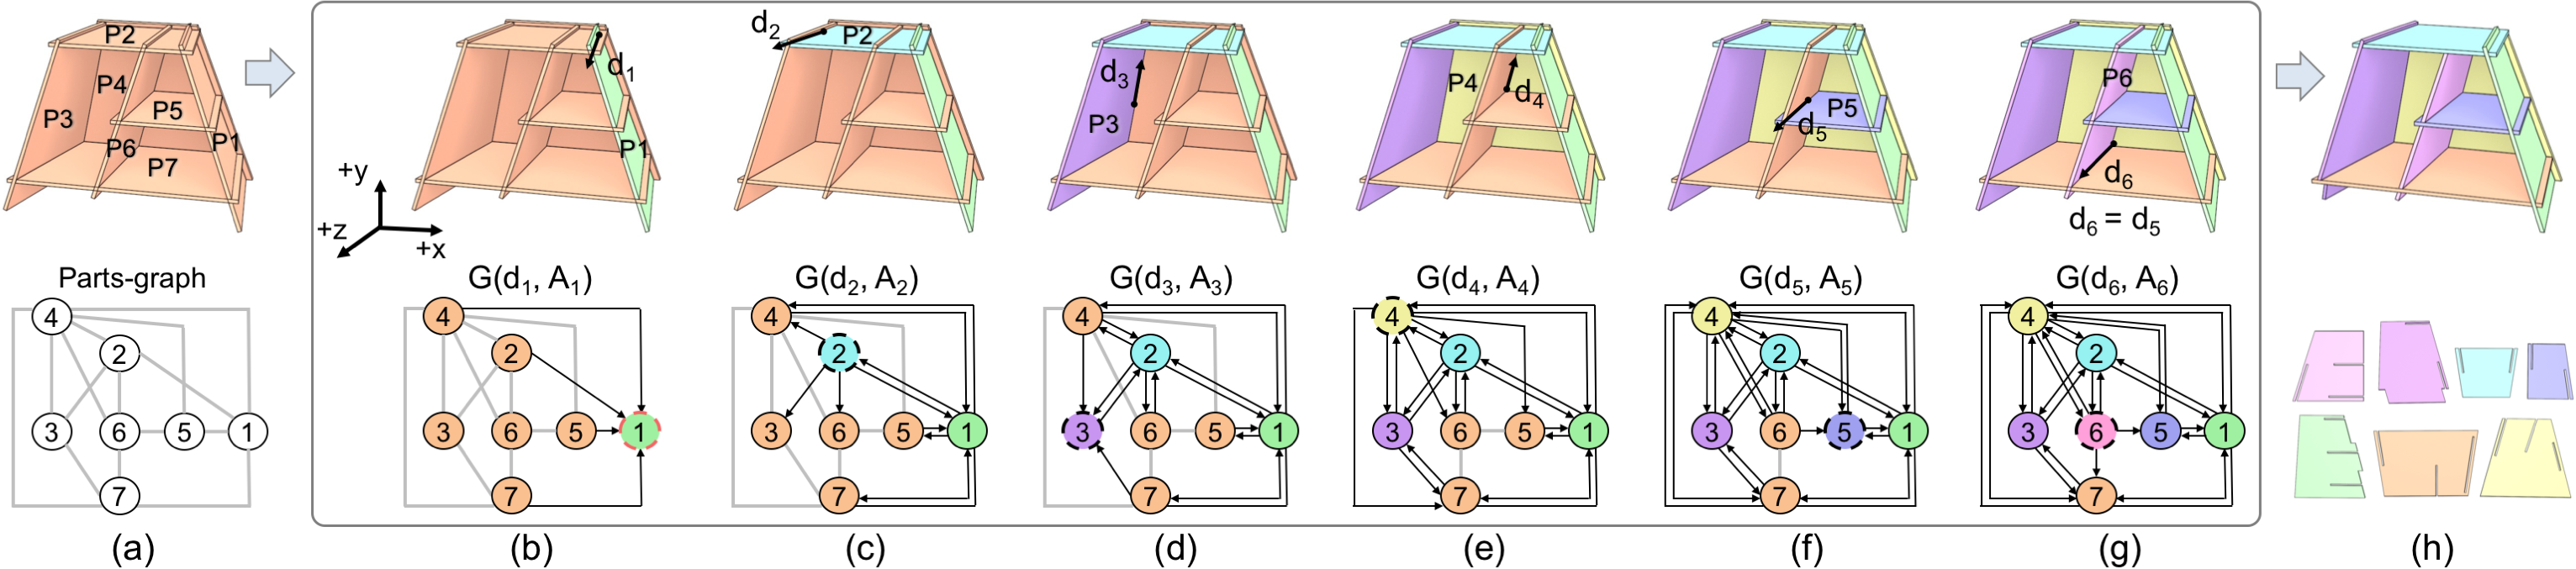
\includegraphics[width=17.75cm]{images/Application_Plate_Cabinet.png}
	\vspace*{-3.5mm}
	\caption{Design of a 7-part interlocking \textsc{Cabinet} by our approach.
		(a) Input design and parts-graph.
		(b-g) The iterative procedure to plan the joints, where the removal direction $d_i$ of $P_i$ is shown in the top and
		the active DBG $G(d_i, A_i)$ is shown at the bottom.
		All orange nodes in each DBG form $R_i$ and the node with dashed boundary is $P_i$.
		(h) The interlocking result and the parts.}
	\vspace*{-2.0mm}
	\label{fig:Application_Plate_Cabinet}
\end{figure*}

\subsection{Interlocking Voxelized Structures}
\label{subsec:puzzle}

Given a voxelized shape and a desired number of parts $N$ as input, our goal here is to decompose the voxel set into a collection of parts that form an interlocking assembly~\cite{Song-2012-InterCubes}.
Figure~\ref{fig:Application_Puzzle_Cube} shows our iterative design process for creating a 9-piece $4\times 4 \times 4$ interlocking {\textsc{Cube}}.
%Our approach have been detailed in Section~\ref{sec:approach}.
%Note that our approach cannot create puzzles with large $N$ may from an input model with relatively small number of voxels.
%For example, our approach cannot find a 10-piece $4\times 4 \times 4$ interlocking {\textsc{Cube}}.

The major difference between our approach and~\cite{Song-2012-InterCubes} is the graph design of $P_i$ and $R_i$ to ensure interlocking of $\mathbf{A}_i$. Our approach makes use of all previous pieces $\{P_1, ..., P_{i-1}\}$ to immobilize $P_i$ and $R_i$.  (i.e., form a cycle in each $\{G(d, A_i)\}$; see Figure~\ref{fig:Framework_Cycle} and~\ref{fig:Application_Puzzle_Cube}), while~\cite{Song-2012-InterCubes} only relies on $P_{i-1}$ to immobilize $P_i$ and $R_i$ (i.e., form a 2-part or 3-part cycle in the DBGs; see Figure~\ref{fig:Application_Puzzle_Model}).
Note that our approach can easily generate recursive interlocking puzzles as~\cite{Song-2012-InterCubes} by constraining our graph design as shown in Figure~\ref{fig:Application_Puzzle_Model}.

\begin{figure}[!t]
	\centering
	%\vspace*{-3.5mm}
	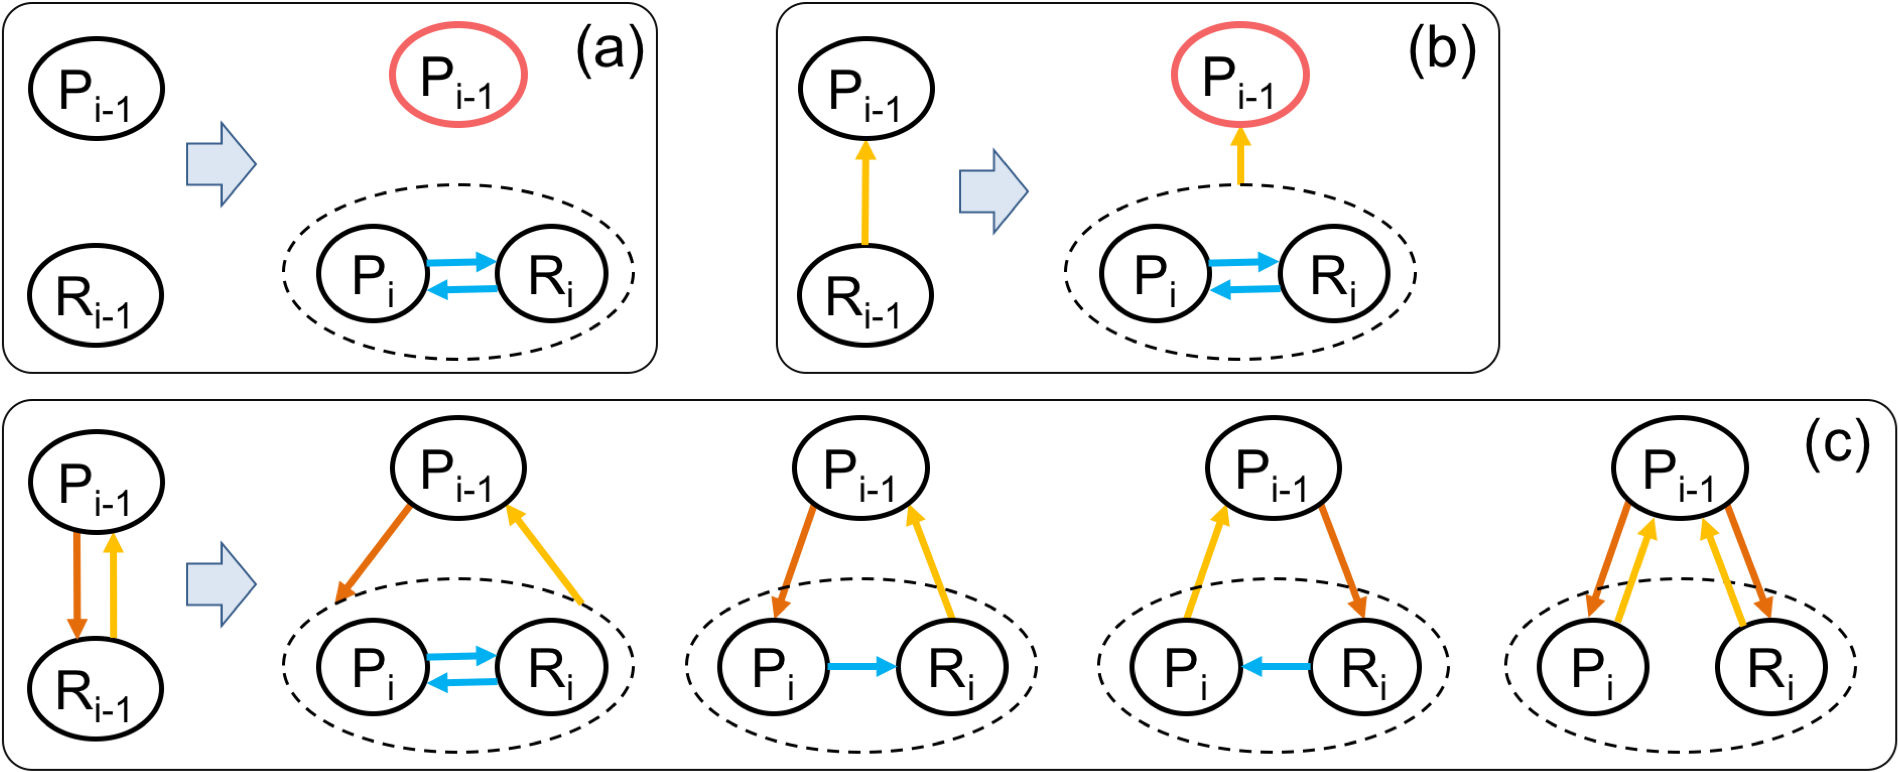
\includegraphics[width=8.40cm]{images/Application_Puzzle_Model.png}
	\vspace*{-2.5mm}
	\caption{
		Illustration of the model of~\cite{Song-2012-InterCubes} based on our DBG-based representation. This approach achieves global interlocking of $A_n$ by requiring every $[P_{i-1}, P_i, R_i]$ ($2 \leq i\leq n$) to form a local interlocking group with $P_{i-1}$ as the key.
		In detail, $P_{i-1}$ and $R_{i-1}$ in $G(d, A_{i-1})$ are possible to have (a) zero, (b) one, and (c) two directed edges.
		%(a) This case is not supported in~\cite{Song-2012-InterCubes} since every part is movable in $[P_{i-1}, P_i, R_i]$ and the approach cannot use any other existing $P_j$ to create blocking relations; 
		%after the partitioning of $R_{i-1}$;
		(a\&b) $P_i$ and $R_i$ are immobilized in a 2-part cycle $[P_i, R_i]$;
		% while the local key $P_{i-1}$ is movable along $d$ in $[P_{i-1}, P_i, R_i]$.
		(c) $P_i$ and $R_i$ are immobilized in either a 2-part cycle $[P_i, R_i]$, $[P_{i-1}, P_i]$, $[P_{i-1}, R_i]$, or a 3-part cycle $[P_{i-1}, P_i, R_i]$.
		%where the rightmost subcase will not happen since $P_i$ and $R_i$ should have at lease one edge.
	}
	\vspace*{-4.0mm}
	\label{fig:Application_Puzzle_Model}
\end{figure}




%Due to this reason, our designed puzzles are interlocking only at the final assembly state while those by~\cite{Song-2012-InterCubes} are interlocking at each intermediate assembly state (i.e., recursive interlocking).
%A good property of recursive interlocking puzzles is that they can be assembled with no or very few supports.
%On the other hand, this property results in strict constraint on the geometry realization, restricting the flexibility of designing interlocking puzzles. 
%

% since each piece locks the successive pieces. 
%\Mark{This could be interpreted as an advantage of your previous approach. It sounds like it would be better for assembly if all stages are interlocking. We should probably highlight the drawbacks of this again.}
%Recursive interlocking puzzles can be assembled with no or very few supports since each intermediate assembly of puzzle pieces remains steady due to interlocking.
 
%Figure~\ref{fig:Application_Puzzle_Cube} compares two 8-piece interlocking cubes designed by our approach and~\cite{Song-2012-InterCubes}, where our constructed cycles in the DBGs have much larger variations than those of~\cite{Song-2012-InterCubes}. 


\begin{figure}[!b]
	\centering
	\vspace*{-3.5mm}
	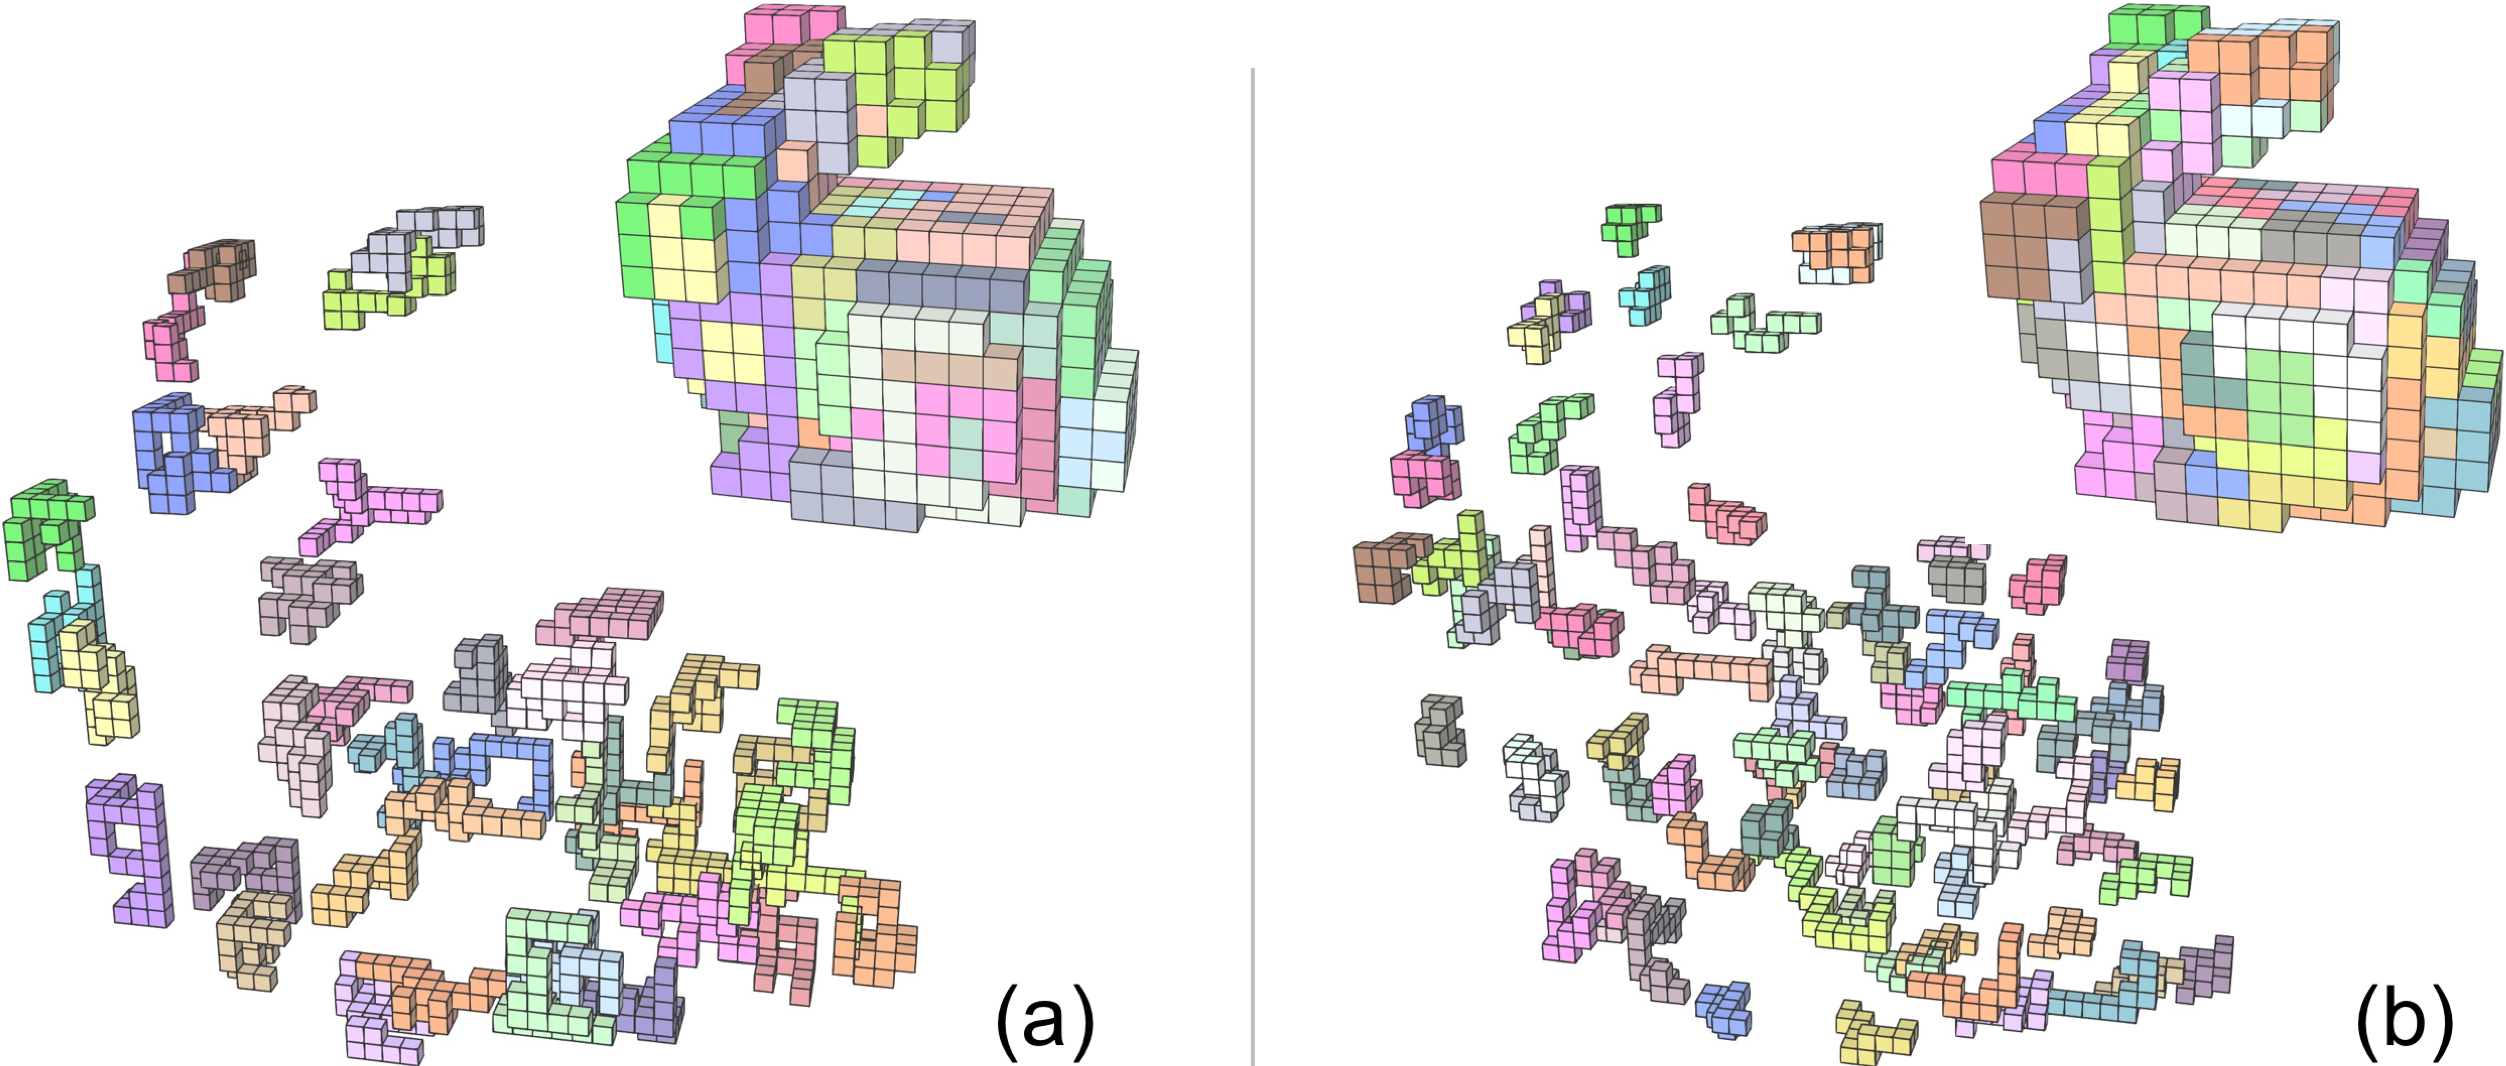
\includegraphics[width=8.20cm]{images/Result_Puzzle_Bunny.png}
	\vspace*{-2.5mm}
	\caption{
		Interlocking {\textsc Bunny}s  (966 voxels). Our method can find assemblies with a large number of parts:  (a)  maximally 40 pieces can be found by the method of~\cite{Song-2012-InterCubes}; (b) 80 pieces using our approach.	
		%Exploded puzzle pieces ($N=40$ in (a) and $N=80$ in (b)) are shown on the left.
	}
	%\vspace*{-4.0mm}
	\label{fig:Result_Puzzle_Bunny}
\end{figure}


%Song et al.~\shortcite{Song-2012-InterCubes} proposes an iterative approach to design recursive interlocking puzzles from a given voxelized shape, where the assembly of puzzle pieces (with at least three pieces) remains interlocking after the sequential removal of pieces.
%A formal model is proposed to ensure global interlocking of all extracted puzzle pieces (i.e., $A_i$) by enforcing local interlocking requirement on every three consecutive intermediate puzzle pieces (i.e., $[P_{i-1}, P_i, R_i]$).  

%We also iteratively construct the puzzle pieces as~\cite{Song-2012-InterCubes}.
% by partitioning each $R_{i-1}$ into $P_i$ and $R_i$.

However, exploiting all existing blocking relations to immobilize $P_i$ and $R_i$ provides significantly more degrees of freedom for designing interlocking assemblies. This allows us to incorporate additional design goals, for example on part appearance as for the {\textsc{Cartoon Dog}} in Figure~\ref{fig:teaser}. Here we impose constraints that avoid cutting seams across geometric features, so that eyes, ears, nose, and tail are each assigned to a single assembly piece.
In addition, as shown in Figure~\ref{fig:Result_Puzzle_Bunny}, our approach can find interlocking assemblies with significantly more parts than~\cite{Song-2012-InterCubes} for the same input.




%First, our approach can generate a significantly larger number of conceptual designs that can be tried at the geometric realization stage.
%This significantly reduces constraint on the geometric realization of the pieces, making it possible to generate interlocking results that cannot be achieved by~\cite{Song-2012-InterCubes}.



%%%%%%%%%%%%%%%%%%%%%%%%%%%%%%%%%%%%%%%%%%%%%%%%
% 2. Interlocking Furniture
%%%%%%%%%%%%%%%%%%%%%%%%%%%%%%%%%%%%%%%%%%%%%%%%


\subsection{Interlocking Plate Structures}
\label{subsec:furniture}

% Problem formulation
%Our framework can be used to design interlocking furniture, in which parts interlock with one another to form a steady assembly.
%Our input is a furniture design represented as a set of simple 3D parts, where adjacent parts may contact or intersect.
%Our goal is to make the furniture interlocking by planning a network of joints between adjacent parts and further modifying the 3D parts with appropriate joint geometry accordingly.
%Similar to~\cite{Fu-2015-Furniture},  we consider parts that are orthogonally connected, and joints that connect a pair of parts and restrict each part to move along a specific axial direction;  see Figure~\ref{fig:Joints}.

 \begin{figure}[!t]
	\centering
	%\vspace*{-3.5mm}
	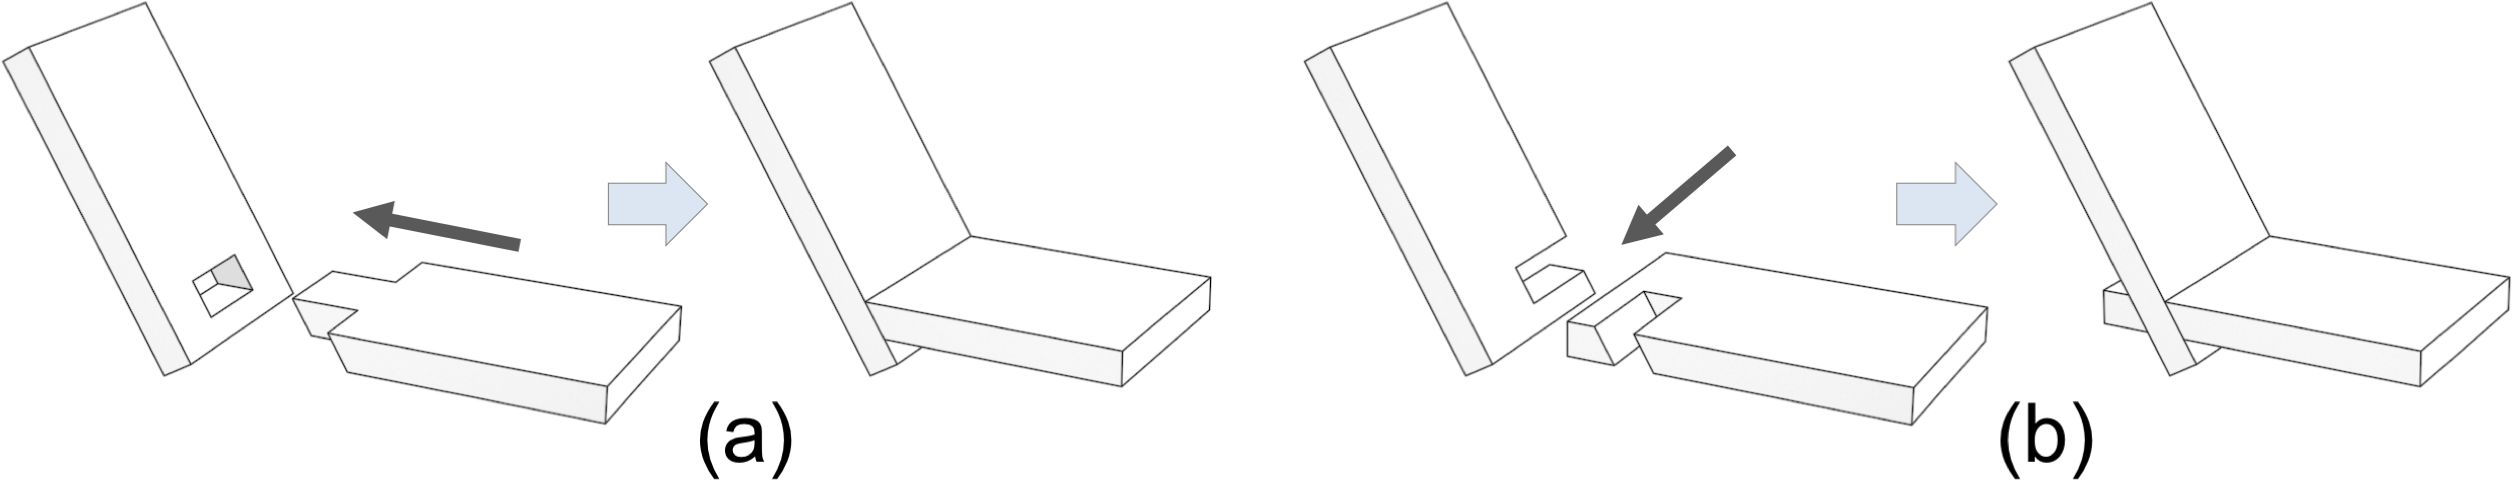
\includegraphics[width=8.45cm]{images/Application_Plate_Joints.png}
	\vspace*{-2.5mm}
	\caption{Variants of (a) mortise-and-tenon joints and (b) halved joints that support non-orthogonal part connection with surface contact.
		%\Mark{Shouldn't we just use (a) and (b)? No need to separate the figures more, I think.}
		%The green arrow shows the possible moving direction of the blue part.
	}
	\vspace*{-4.0mm}
	\label{fig:Application_Plate_Joints}
\end{figure}
 
A second class of assemblies that we can create with our approach are interlocking plate structures that have applications in furniture design or architecture, for example.
These assemblies differ in two main ways from the voxelized assemblies described above.
First, the geometry of parts and their connections are predefined. We model part connections with an undirected {\em parts-graph}, in which nodes represent parts, and edges connect two contacting/intersecting parts; see Figure~\ref{fig:Application_Plate_Cabinet}(a). 
Blocking relations can only be constructed between parts connected in the parts-graph.
The dual of a {\em parts-graph} is a {\em joints-graph}, where nodes represent joints and edges represent parts; see Figure~\ref{fig:Application_Frame_Cube}(a). 
Second, we use a set of predefined joint geometries to impose blocking relations between each pair of adjacent parts in the structure. 
Specifically, we consider mortise-and-tenon, halved, and dovetail joints that restrict each part to move along a single direction; see Figure~\ref{fig:Joints}.
To support non-orthogonal part connection, we consider suitable variants of mortise-and-tenon and halved joints;
\setlength{\columnsep}{12pt}
\begin{wrapfigure}{r}{0.32\columnwidth}
	\vspace{-12pt}
	\centering
	\hspace{-8pt}
	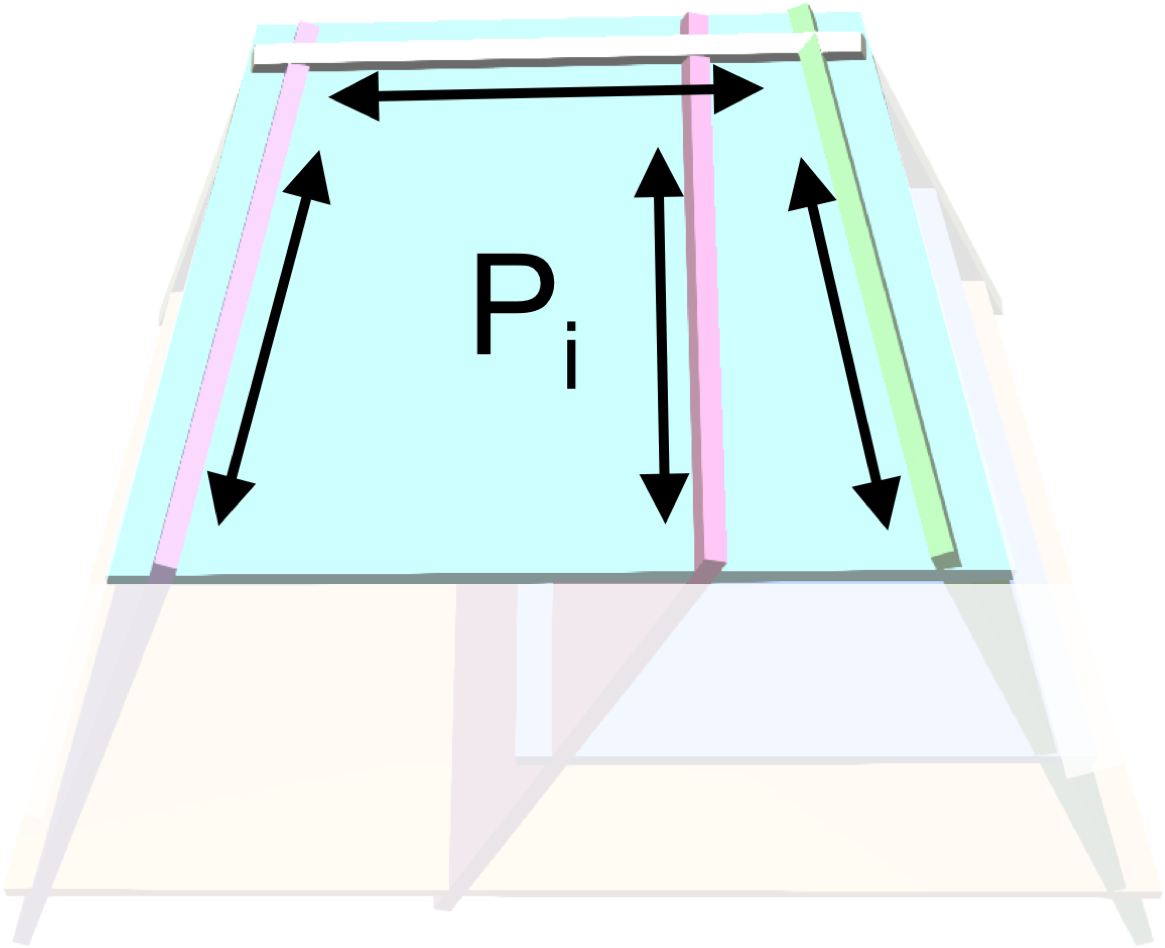
\includegraphics[width=0.30\columnwidth]{images/Application_Plate_Direction.png}
	\vspace{-11pt}
\end{wrapfigure}
see Figure~\ref{fig:Application_Plate_Joints}.
In plate structures,  the edge vectors shared between each part $P_i$ and its adjacent parts indicate the base directions $\{d\}$ (see the arrows in the inset for examples), which degenerate into six axial directions for structures where parts are orthogonally connected; see Figure~\ref{fig:Application_Furniture_Table}(a).

\if 0
To address above specifics of interlocking plate structures, we have the following adaptations to our framework.
First, we iteratively select a single part $P_i$  from the input, and consider the set of unselected parts as $R_i$.
At each iteration, our goal is to select a part from $R_{i-1}$ as $P_i$ and choose a removal direction of $P_i$ in $[P_i, R_i]$ denoted as $d_i$ such that $\mathbf{A}_i$ ($i\geq$2) is interlocking. 
\fi

%For a non-orthogonal HV joint, the removal direction is $\vec{e}$, which is an edge vector shared between parts.
%And we may choose between $+\vec{e}$ and $-\vec{e}$ when planning the joint; see Figure~\ref{fig:Application_Plate_Joints}(a\&b).
%For a non-orthogonal MT joint, the removal direction $\vec{d_t}$ of the tenon part is perpendicular to the part's normal; see Figure~\ref{fig:Application_Plate_Joints}(c\&d).

%For a halved joint the removal direction is the vector shared between parts that can be chosen in either orientation when planning the joint. 
%For a mortise-tenon joint, the removal direction of the tenon part is perpendicular to the part's normal.

%which allow parts to be non-orthogonally connected along planar surfaces

%
% In the three base DBGs, planning a joint between $P_i$ and $P_j$ that restricts $P_i$ to move along $d_i$ relative to $P_j$ will create a directed edge between the two parts in $G(d_i, A)$ and two directed edges in the other two base DBGs.
 %
 % Customized framework
 %
 

 
 \begin{figure*}[!t]
 	\centering
 	%\vspace*{-3.5mm}
 	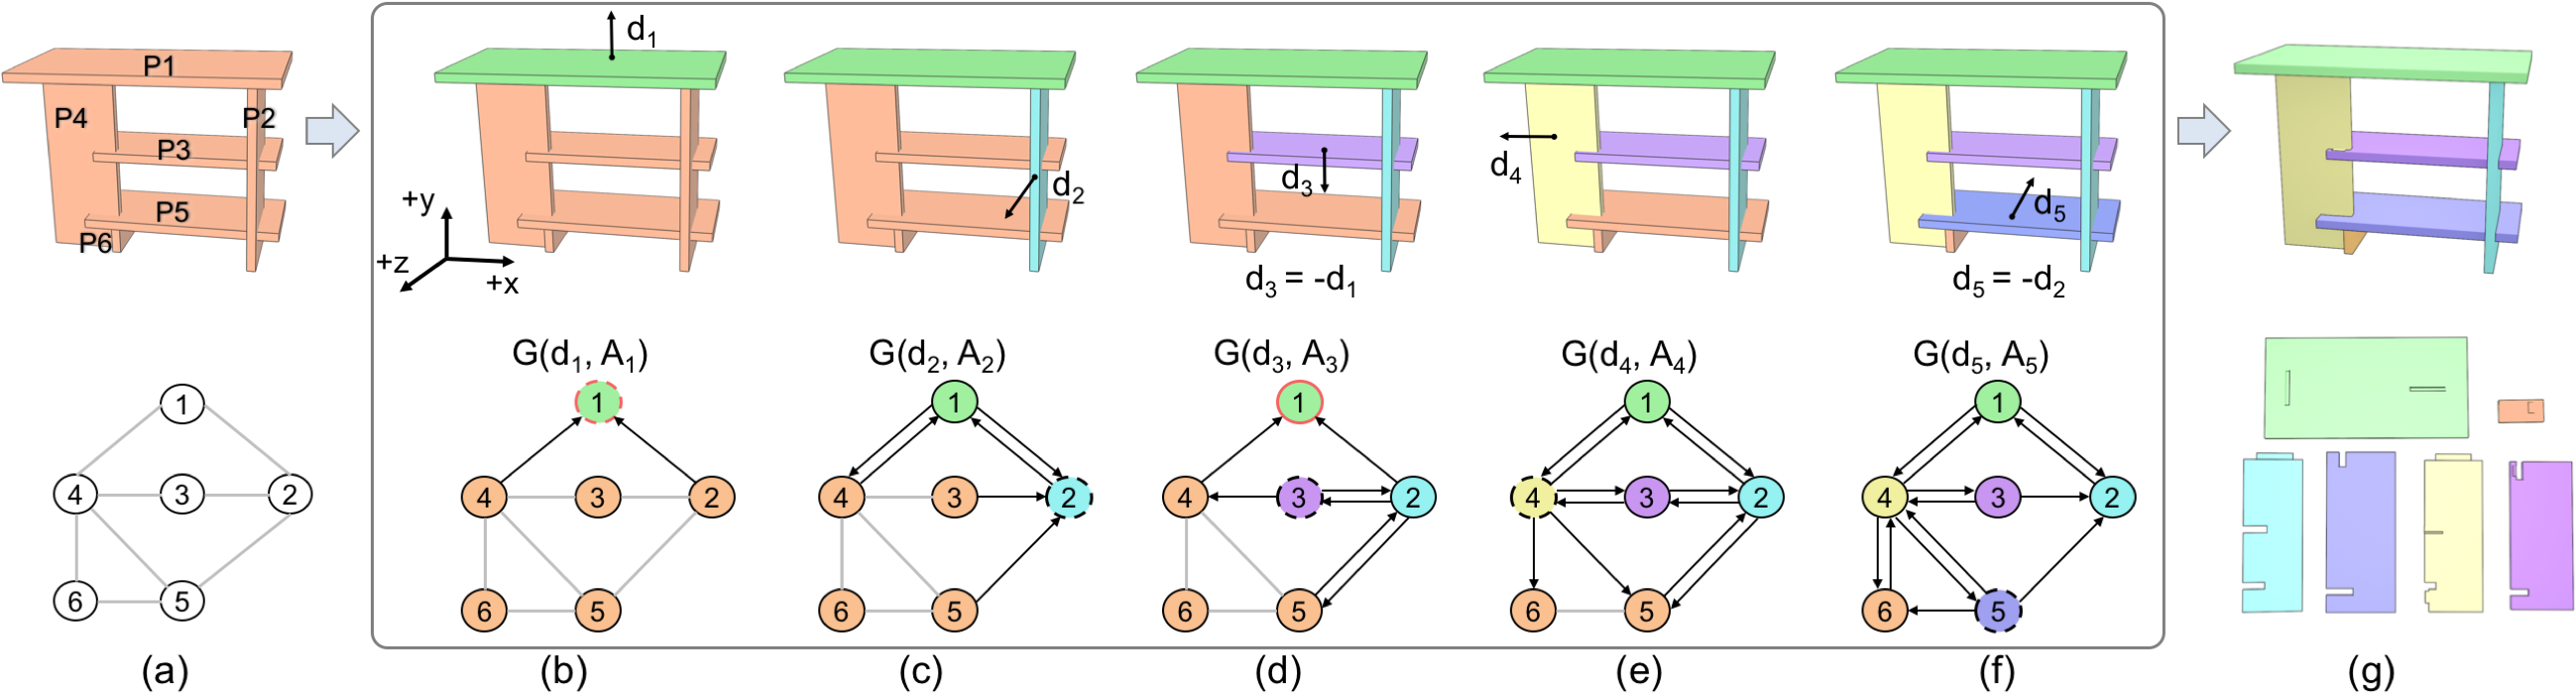
\includegraphics[width=17.75cm]{images/Application_Furniture_Table.png}
 	\vspace*{-3.5mm}
 	\caption{Design of a 6-part interlocking \textsc{Table} with orthogonal joints.
 		(a) Input design and parts-graph.
 		(b-f) The iterative procedure to plan the joints.
 		(g) The interlocking result and the parts.
 		%\Mark{I like this example for illustration. But people could argue that such a design, one could easily do by hand. We should also have examples where the complexity is to high to be able to figure things out manually.}
 		%\Peng{We have more complex examples in Result section; Without our iterative design approach, designing an interlocking furniture with a few parts would be a difficult problem.}
 	}
 	\vspace*{-2.0mm}
 	\label{fig:Application_Furniture_Table}
 \end{figure*}
 
To address the above specifics of interlocking plate structures, we have the following adaptations compared to the voxelized structures.
First, instead of decomposing $R_{i-1}$ into $P_i$ and $R_i$, we iteratively select a single part $P_i$  from the input, and consider the set of unselected parts as $R_i$; see Figure~\ref{fig:Application_Plate_Cabinet}(b-g).
Second, rather than constructing the geometry of $P_i$ and $R_i$, we construct joints between $P_i$ and each part in $R_i$ that are connected with $P_i$ in the parts-graph denoted as $R_i^{'}$ such that $\mathbf{A}_i$ ($i\geq$2) is interlocking.
Since all our employed joints allow a single removal direction of the parts, the removal direction of $P_i$ in $[P_i, R_i]$ denoted as $d_i$ completely defines the joints to be constructed beween $P_i$ and each part in $R_i^{'}$.
Third, to achieve interlocking, we only need to ensure that the {\em active base DBG} $G(d_i, A_i)$ is strongly connected; see DBGs in Figure~\ref{fig:Application_Plate_Cabinet}(b-g).
The other base DBGs should remain strongly connected since the newly introduced joints only allow part moving along $d_i$ but not the other base directions.

%This is because making $P_i$ movable along $d_i$ in $[P_i, R_i]$ will create two directed edges between $P_i$ and each part in $R_i$ for all the other base DBGs.
%These specifics of interlocking plate structures require the following adaptations to our framework.
%In detail, we  require the following adaptations to our framework.
 Our iterative approach is detailed as follows:
 \begin{itemize}[leftmargin=*]
\vspace{-0.5mm}
\item 
{\em Iterative Design Framework.} \
 Starting from the key $P_1$, we iteratively select a single part $P_i$  from parts in $R_{i-1}$.
We avoid selecting $P_i$ that is a cut point in the remaining parts-graph of $R_{i-1}$ in order to keep the geometry of $R_i$ simply connected.
Once $P_i$ is selected, our task is to select $d_i$ from the edge vectors $\{e_i\}$ shared between $P_i$ and its adjacent parts.


%The base directions of $\mathbf{A_i}$ are $\{d\} = \{d_1, ..., d_i\}$, where $d_j$ ($1 \leq  j \leq i$) is the removal direction of $P_j$ in $[P_j, R_j]$.
%Note that if $d_j = d_k$ ($j\neq k$, $d_j \in \{d\}$, $d_k \in \{d\}$), $G(d_j, A_i)$ and $G(d_k, A_i)$ are actually the same DBG.

 %The selection of $P_i$ can be specified by the user or follow certain criteria, e.g., from top to bottom.


%Here, we find the candidates of $d_i$ following the joint analysis technique in~\cite{Fu-2015-Furniture}; e.g., the candidates of $d_1$ in Figure~\ref{fig:Application_Furniture_Table}(b) are $\{+x, -x, +y, +z, -z\}$.
%, $P_i$ is separable from $R_i$ in $[P_i, R_i]$, and $[P_1, ..., P_i, R_i]$ is interlocking.
 
 \vspace{1mm}
\item 
{\em Generating the key.} \
Generally, we select $P_1$ as the part with the most parallel joint directions, and use this direction as $P_1$'s removal direction $d_1$ to facilitate joint construction on the key; see Figure~\ref{fig:Application_Plate_Cabinet}(b).
This is because we create a halved joint for the edge that is parallel to $d_1$, a mortise-tenon joint for the edge that is nearly perpendicular to $d_1$ (angle within $[45^\circ, 135^\circ]$), and an empty joint for the other edges.  
%For orthogonal structures, $P_1$ and $d_1$ are usually selected as the topmost part with upward $d_1$ (immobilized by gravity) or the bottom part with downward $d_1$ (immobilized by the ground).
After selecting $P_1$ and $d_1$, we plan a joint between $P_1$ and each part in $R_1^{'}$ (e.g.,  $R_1^{'} = \{P_2, P_4, P_5, P_7\}$ in Figure~\ref{fig:Application_Plate_Cabinet}(b)) such that $P_1$ is only movable along $d_1$.


%Depending on the application, the user might prefer other key parts, e.g. the topmost part with upward $d_1$ (immobilized by gravity) or the bottom part with downward $d_1$ (immobilized by the ground). These can be selected accordingly in our user interface.
%We find all parts that connect with $P_1$ in the parts-graph, and plan a joint between each part and $P_1$ such that $P_1$ is only movable along $d_1$; see Figure~\ref{fig:Application_Furniture_Table}(b).
 
 \vspace{1mm}
\item 
 {\em Generating $P_i$ and $R_i$ ($i>1$).} \
 At the graph design stage, we need to select $d_i$ from $\{e_i\}$ such that $G(d_i, A_i)$ is strongly connected, which can be classified into two cases.
 The first case is that $\pm d_i \notin \{d_1, ..., d_{i-1} \}$. 
 For this case, we build $G(d_i, A_i)$ by converting each undirected edge among $\{P_1, ..., P_{i-1}, R_{i-1}\}$ in the parts-graph into two directed edges and adding a single directed edge between $P_i$ and each part in $R_i^{'}$. 
 The $G(d_i, A_i)$ should be strongly connected by default; see Figure~\ref{fig:Application_Plate_Cabinet}(c).
 The second case is that $d_i$ or $-d_i$ $\in \{d_1, ..., d_{i-1} \}$, say $d_i = d_k$ ($1\leq k \leq i-1$).
$G(d_i, A_i)$ inherits all blocking directions from $G(d_k, A_{i-1})$ and we add a single directed edge between $P_i$ and each part in $R_i^{'}$.
We try each of the two directions of the edge and accept $d_i$ if $G(d_i, A_i)$ is strongly connected; see Figure~\ref{fig:Application_Plate_Cabinet}(g).

 \vspace{0.5mm}
 At the geometry realization stage, we use constructive solid geometry to create the joint geometry of $P_i$ and each part in $R_i^{'}$ according to the joint type selected during the graph design.
We rank the resulting candidates of $\mathbf{A}_i$ in ascending order of the number of empty joints in $\mathbf{A}_i$.
 %Among all valid conceptual designs, we rank  that results in a fewer number of empty joints.
 %  Given a conceptual design, we create the joint geometry following the approach in Subsec~\ref{subsec:furniture}.

 \end{itemize}

Figure~\ref{fig:Application_Plate_Cabinet}(h) shows an interlocking \textsc{Cabinet} designed by our approach.
Besides furniture, plate structures can also be used to approximate a free form shape; see the 33-part \textsc{Lizard}  in Figure~\ref{fig:teaser} for an example.
In the special case of orthogonal joints, our approach generalizes the furniture design work of~\cite{Fu-2015-Furniture}; see Figure~\ref{fig:Application_Furniture_Table} for an example.
In particular, Fu et al.~\shortcite{Fu-2015-Furniture} focus on furniture design with 3- or 4-part cyclic substructures since their approach requires these substructures to construct LIGs.
In contrast, our approach does not have such a limitation; see the \textsc{Bookshelf} result with four 6-part cyclic substructures in Figure~\ref{fig:teaser}.

Lastly, inspired by our DBG-based representation, we find that a parts-graph with a cut point cannot be interlocking, no matter what kinds of joints are planned; see Figure~\ref{fig:Result_Furniture_Chair}(left) for an example and supplementary material for the proof.
This observation allows us to modify a given input to make it possible to be interlocking by adding a minimal number of new parts in the parts-graph in oder to remove the cut point; see Figure~\ref{fig:Result_Furniture_Chair}(right) for an example.

\begin{figure}[!t]
	\centering
	%\vspace*{-3.5mm}
	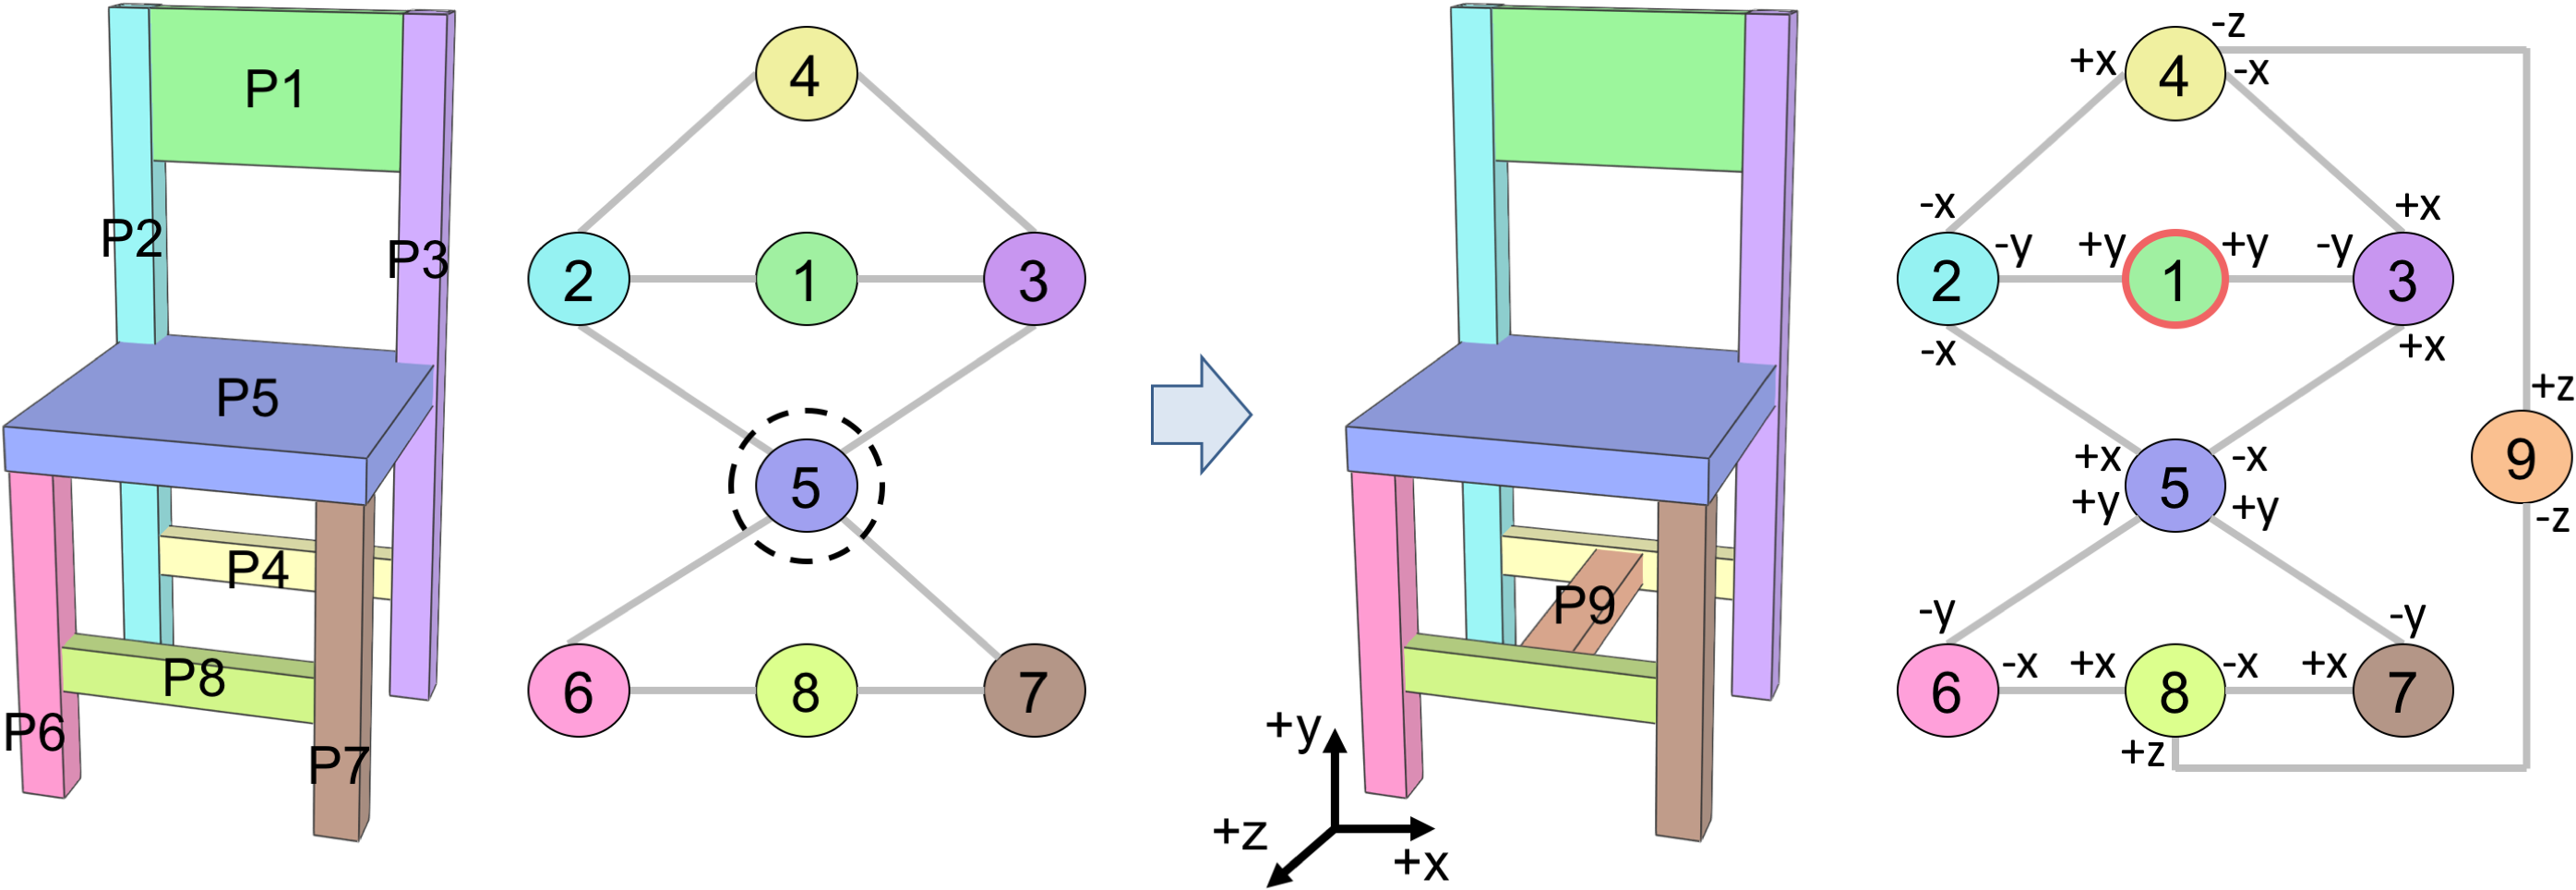
\includegraphics[width=8.45cm]{images/Result_Furniture_Chair.png}
	\vspace*{-2.5mm}
	\caption{
		Left: a {\textsc Chair} and its parts-graph, where a cut point (i.e., $P_5$) exists.
		Right: after adding a new part (i.e., $P_9$), our approach can generate an interlocking joint configuration, where the axial removal direction allowed by each joint is shown in the corresponding edge in the parts-graph. 
	}
	\vspace*{-4.5mm}
	\label{fig:Result_Furniture_Chair}
\end{figure}







\if 0
 Since our assembly supports non-orthogonal joints, we maintain a {\em dynamic set} of base DBGs denoted as $\{G(d, A_i)\}$ for each iteration of generating $\mathbf{A_i}$. The base directions of $\mathbf{A_i}$ are $\{d\} = \{d_1, ..., d_i\}$, where $d_j$ ($1 \leq  j \leq i$) is the removal direction of $P_j$.
Note that if $d_j = d_k$ ($j\neq k$, $d_j \in \{d\}$, $d_k \in \{d\}$), then $G(d_j, A_i)$ and $G(d_k, A_i)$ are actually the same DBG. For example, if all joint directions are axis-aligned as in Figure~\ref{fig:Application_Furniture_Table}, we end up with only three base DBGs.


Figures~\ref{fig:Application_Furniture_Table} and~\ref{fig:Application_Plate_Cabinet} show examples of interlocking plate structures. 

Figures~\ref{fig:Application_Furniture_Table}(g) shows the joint configuration planned by our approach, as well as geometry of each modified part.
Although both our approach and~\cite{Fu-2015-Furniture} can generate results on this input model, Section~\ref{sec:results} will show some of our results that cannot be achieved by~\cite{Fu-2015-Furniture}.


\fi




%%%%%%%%%%%%%%%%%%%%%%%%%%%%%%%%%%%%%%%%%%%%%%%%
% 3. Interlocking Frame Structures
%%%%%%%%%%%%%%%%%%%%%%%%%%%%%%%%%%%%%%%%%%%%%%%%

  \begin{figure*}[!t]
	\centering
	%\vspace*{-3.5mm}
	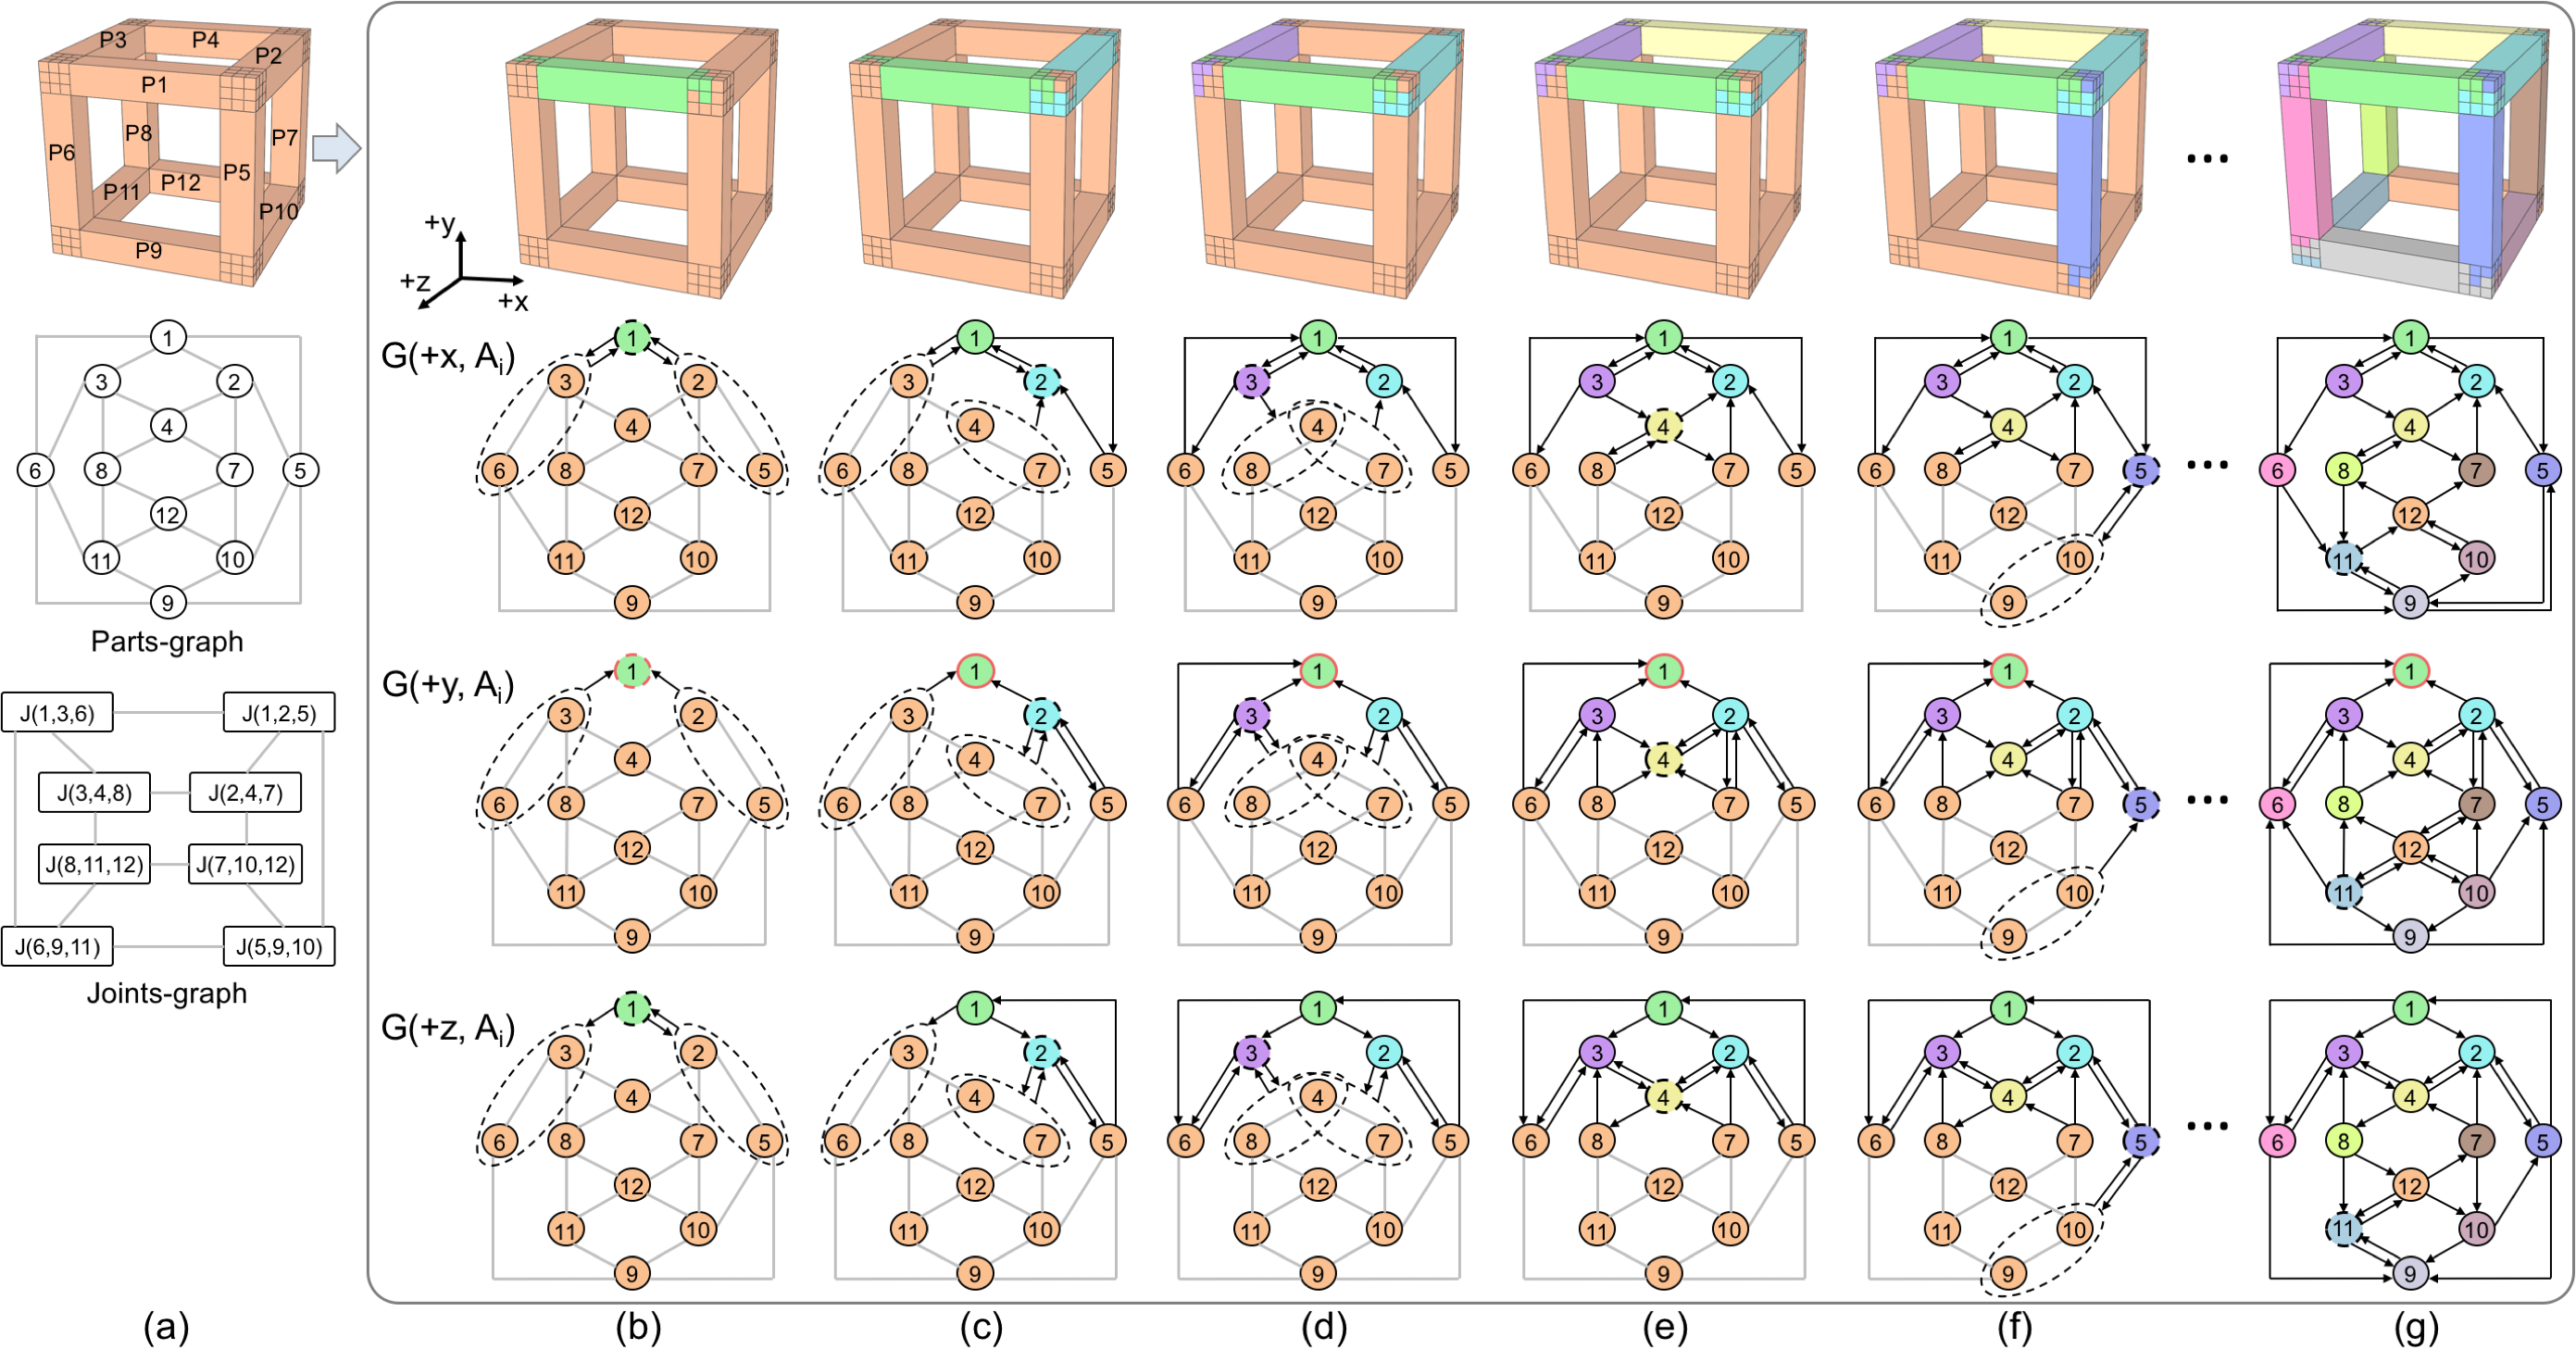
\includegraphics[width=17.75cm]{images/Application_Frame_Cube.png}
	\vspace*{-3.5mm}
	\caption{Design of a 12-part interlocking \textsc{Frame Cube}.
		(a) Input frame design, parts-graph, and joints-graph.
		(b-f) The iterative procedure to construct the cube joints, where the dashed ellipses highlight the set of parts in $R_i$ that connect with $P_j$ ($j\leq i$) using cube joints.
		% where all orange nodes in each DBG form $R_i$ and the node with dashed boundary is $P_i$.
		(g) The interlocking result.}
	\vspace*{-2.0mm}
	\label{fig:Application_Frame_Cube}
\end{figure*}



\subsection{Interlocking Frame Structures}
\label{subsec:frame}

% Problem formulation
As a new class of interlocking assembly, we propose  {\em interlocking frame structures} that can be considered a hybrid of the voxelized and the plate assemblies. A frame structure is a network of beams joined to represent a desired target shape. As input we assume a 3D polygonal mesh, where each edge represents a beam and each vertex represents a joint.
%Different from the furniture application, joint in a frame structure usually connects more than two parts, making traditional wooden joints infeasible.
%Thus, we propose to connect the beams with {\em puzzle joints}.
%Our goal is to construct a network of joints among all the beams to make the frame structure interlocking.

% Major different from furniture design
Compared with the plate assemblies, this application has two more challenges.
First, frame structures require connecting more than two parts at a joint, making traditional woodworking joints unsuitable; see the joints-graph in Figure~\ref{fig:Application_Frame_Cube}(a).
Thus, we propose to connect the beams with cube-shaped {\em voxel joints}.
To make the problem tractable, we assume that each face of the cube joint connects to at most one beam at the center voxel, and thus each cube connects at most six beams (i.e., valence of the input mesh should be at most 6).
Second, we need to individually optimize the geometry of each cube joint. We place an axis-aligned $3 \times 3 \times 3$ cube at each joint location and partition the cubes into pieces to restrict the relative movement of the connected beams; see the eight corners of the \textsc{Frame Cube} in Figure~\ref{fig:Application_Frame_Cube}(a). 
%
 % Customized framework
Compared to the plate structures, these specifics require the following adaptations to our framework:
%\vspace*{-2.0mm}
\begin{itemize}[leftmargin=*]
%	\item 
%	{\em Iterative Design Framework.} \	
%	The procedure is the same as that in Subsection~\ref{subsec:furniture}, except that we need to ensure geometric connectivity of each modified part.
%	To achieve this, we preassign the center voxel of the puzzle cube face to the part that is connected to that face.
%	Later, when we assign more voxels to the part at each of its two ends, we ensure that each group of assigned voxels (i.e., integral joint) are simply connected.
	
	\vspace*{1.0mm}
	\item 
	{\em Generating the key.} \
	For the cube joint at each end of $P_1$, we take the voxel preassigned to $P_1$ as a seed and include more voxels to $P_1$ such that it is movable along a singe axial direction following Subsection~\ref{subsec:genKey}.
	Denote the subset of parts that connect with $P_1$ at each end as $S_1^k = \{P_l\}$, where $k \in \{1, 2\}$; see the dashed circles in Figure~\ref{fig:Application_Frame_Cube}(b).
	After constructing $P_1$, we draw directed edges between $P_1$ and each $S_1^k$ in the DBGs accordingly.
	
	\vspace*{1.0mm}
	\item 
	{\em Generating $P_i$ and $R_i$ ($i>1$).} \
	%Denote the subset of parts that connect with $P_i$ at each end as $S_i^k = \{P_l\}$, where $k \in \{1, 2\}$.
	At the graph design stage, we classify parts in each $S_i^k$ into two groups: $\{ \grave{P}_l \}$ where each part is from $\{P_1, ..., P_{i-1} \}$ and $\{ \acute{P}_l\}$ where each part is from $R_i$. 
	If $\{ \acute{P}_l\}$ is empty, the blocking relations within this cube joint are completely defined.
	So the graph design of $P_i$ and $R_i$ can be skipped for this joint; see joint $J(1,2,5)$ in Figure~\ref{fig:Application_Frame_Cube}(f), where $P_i$ = $P_5$, $\{ \grave{P}_l \} = \{P_1, P_2\}$.
	If $\{ \grave{P}_l \}$ is empty, we do not need to distribute external blocking relations in this joint; see joint $J(2,4,7)$ in Figure~\ref{fig:Application_Frame_Cube}(c), where  $P_i$ = $P_2$, $\{ \acute{P}_l \} = \{P_4, P_7\}$.
	Otherwise, we distribute external blocking relations associated with $\{ \grave{P}_l \}$ to $P_i$ and parts in $\{ \acute{P}_l\}$ respectively; see joint $J(1,2,5)$ in Figure~\ref{fig:Application_Frame_Cube}(c).
	%, where $P_i$ = $P_2$, $\{ \grave{P}_l \} = \{P_1\}$,  $\{ \acute{P}_l\} = \{P_5\}$.
	Constructing internal blocking relations is restricted to $P_i$ and parts in $\{ \acute{P}_l\}$ for each $S_i^k$.
	To ensure that $P_i$ is disassemblable in $[P_i, R_i]$, say along $d_i$, we construct a single directed edge between $P_i$ and each part in $\{ \acute{P}_l\}$ for both $S_i^k$ in at least one DBG; see $G(+x, A_2)$ in Figure~\ref{fig:Application_Frame_Cube}(c) for an example.
%	The procedure to find candidates of $d_i$ and ensure interlocking of $\mathbf{A}_i$ conceptually is the same as that in Subsection~\ref{subsec:furniture}.

	%plan exactly the same joint between $P_i$ and each part in $R_i^{'}$; see Figure~\ref{fig:Application_Furniture_Table}(c\&e).
	%To ensure that $[P_1, ..., P_i, R_i]$ is interlocking, we try all possible $d_i$, and select those that result in at least one cycle including both $P_i$ and $R_i$ in each $G(d, A_i)$. 
	%Here, we find the candidates of $d_i$ by employing the joint analysis technique in~\cite{Fu-2015-Furniture}; e.g., the candidates of $d_1$ in Figure~\ref{fig:Application_Furniture_Table}(b) are $\{+x, -x, +y, +z, -z\}$.
	%For example, the candidates of $d_i$ in the inset are ${+x, -x}$. 
	%In particular, to ensure that the conceptual design is realizable in the embedded geometry, we employ the joint analysis technique in~\cite{Fu-2015-Furniture} to find the possible joints (and thus the associated axial direction) that can be deployed at the connection between $P_i$ and each part in $R_i^{'}$. 
	
	%\vspace*{1.0mm}
	%\item 
	%{\em Geometry Realization of $P_i$ and $R_i$.} \
	%Once we find an interlocking configuration (see Figure~\ref{fig:Application_Furniture_Table}(g)), 
	The geometry realization of $P_i$ and $R_i$ is conducted within the cube joint at each end of $P_i$ following the approach in Subsection~\ref{subsec:genPart}; see corners of the \textsc{Frame Cube} in Figure~\ref{fig:Application_Frame_Cube}(c-f).
	% which can be performed very efficiently since each puzzle joint has only 27 voxels.
\end{itemize}

\begin{figure}[!t]
	\centering
	%\vspace*{-3.5mm}
	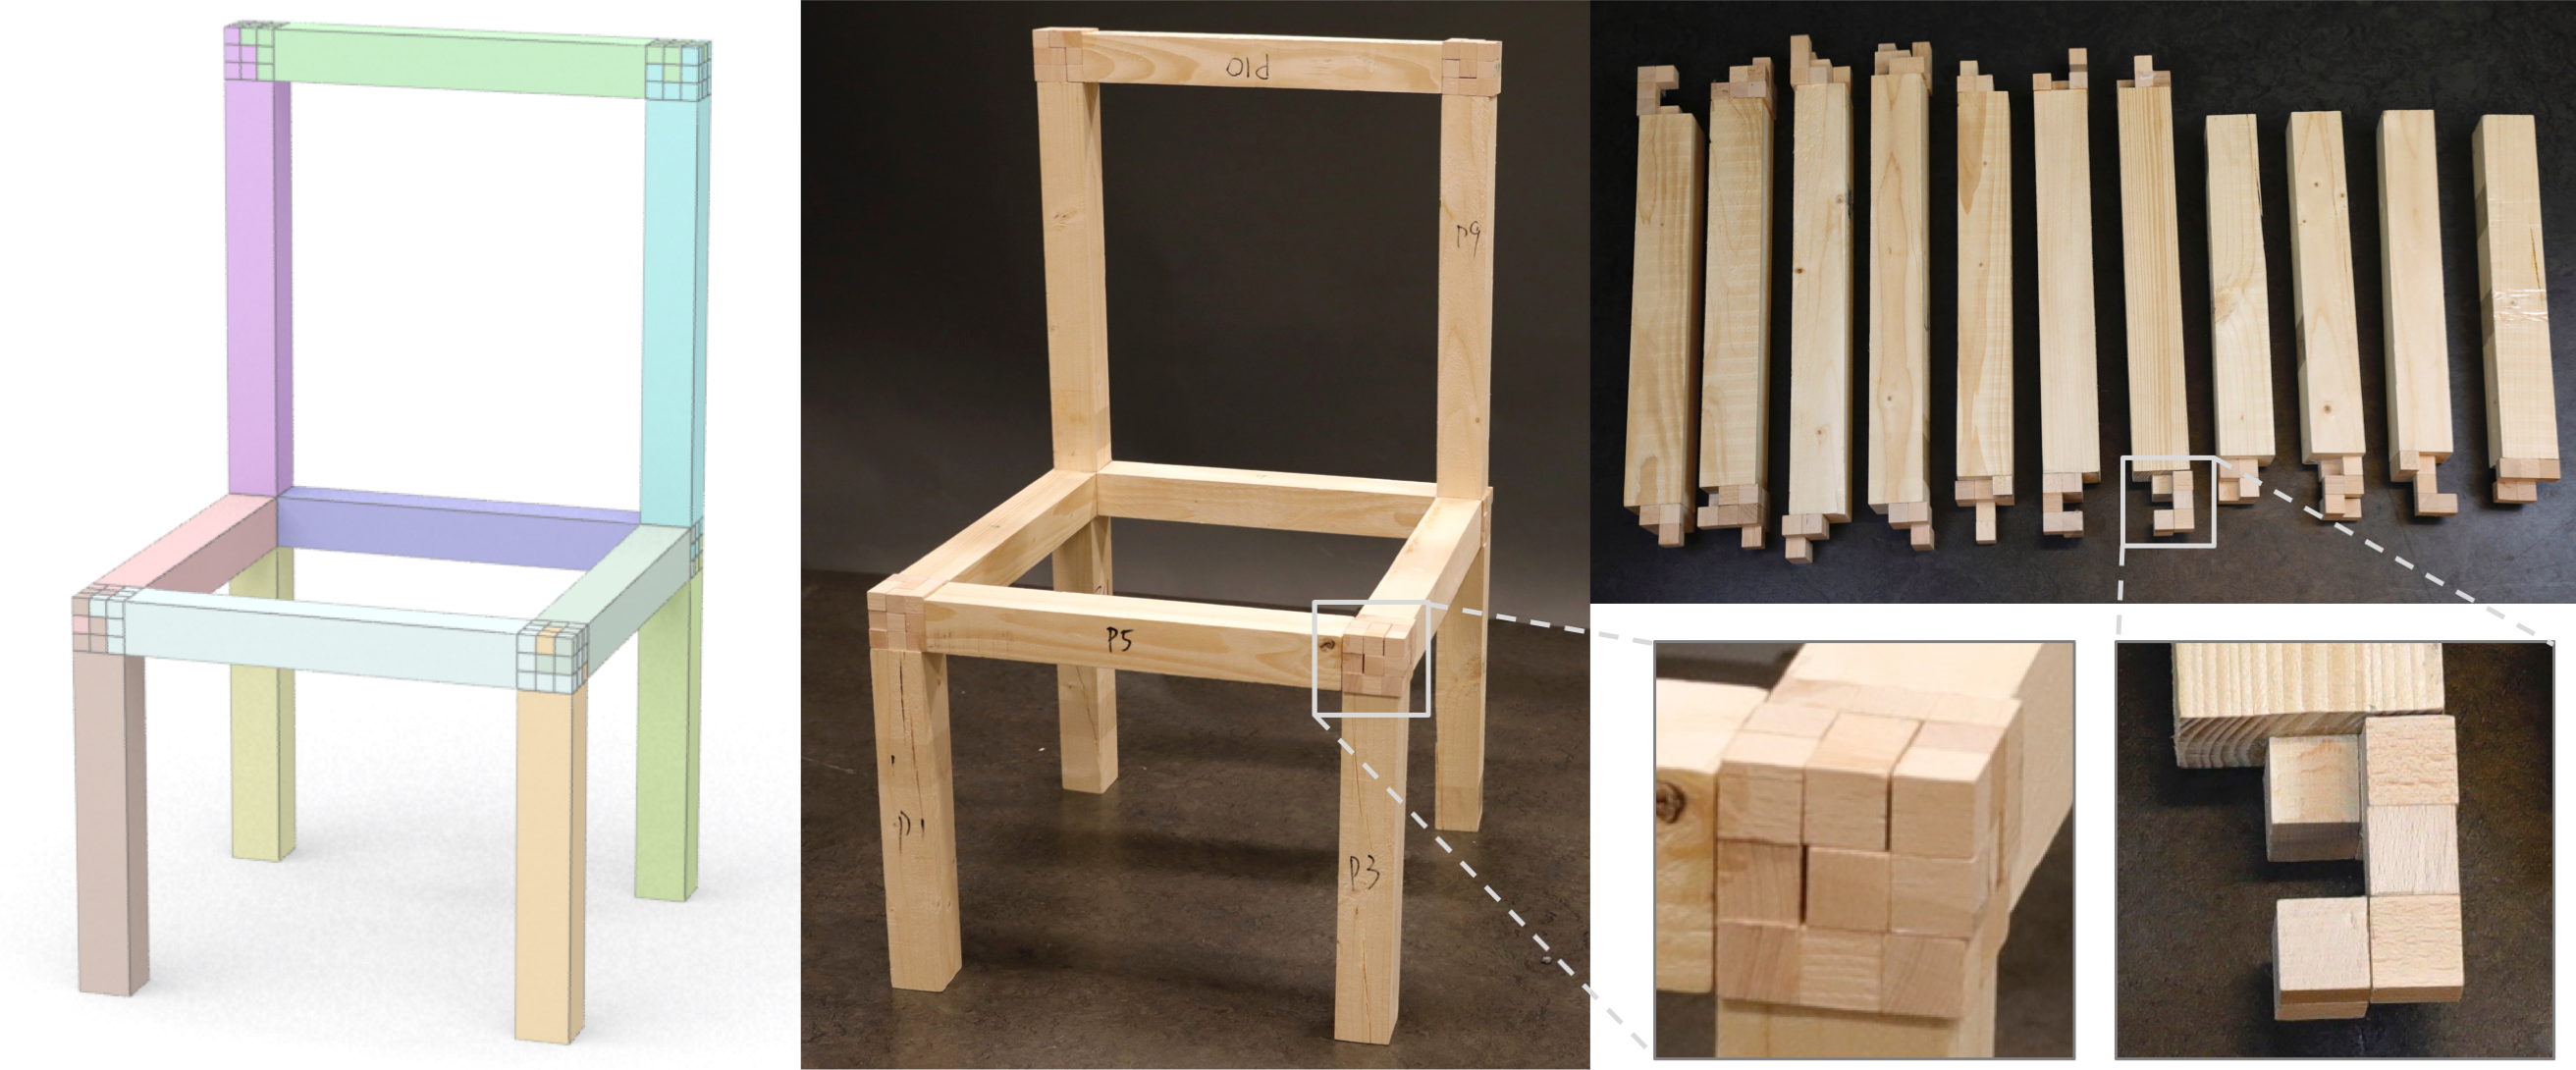
\includegraphics[width=8.45cm]{images/Result_Frame_Physical.png}
	\vspace*{-2.5mm}
	\caption{
		Interlocking $1.0m \times 0.5m \times 0.5m$ {\textsc Frame Chair}. The voxel joints are fabricated by gluing wooden cubes in the spatial arrangement computed by our algorithm. When attached to the corresponding wooden beams, all beams can be connected into a stable interlocking assembly.}
	\vspace*{-4.0mm}
	\label{fig:Result_Frame_Physical}
\end{figure}

Figure~\ref{fig:Application_Frame_Cube}(g) shows the resulting interlocking \textsc{Frame Cube}, in which every three beams joining at a corner are connected by a carefully constructed three-way cube joint. Note that all joints are distinct even though all corners are symmetric. This illustrates how the assembly order dictates the geometry of the joints, more so than the geometry of the parts.

Our approach can generate frame structures with different joint valence, e.g., the valence in the \textsc{Frame Chair} in Figure~\ref{fig:Result_Frame_Physical} can be 2, 3 or 4.
We fabricate this result using wooden pillars and small wooden cubes to validate its steadiness; see supplementary video for the live demo.
Figure~\ref{fig:teaser} shows another \textsc{Flower} result, where curved beams are connected by the cube joints to form an appealing structure.
%Note that the puzzle joints still have to be axial aligned in 3D space to satisfy the part surface contact requirement.
To the best of our knowledge, these are the first {\em single-key} interlocking frame structures.



% that connect beams with puzzle joints.


\subsection{Implementation and Performance}
% \TODO{Add some details of implementation, reference to source code, and some timing statistics.}
Our C++ implementation runs on an iMac with a 4.2GHz CPU and 32GB memory.
In general, the timing performance depends on the input model, the number of parts $N$, and additional design requirements.
Our approach creates interlocking plate structures very efficiently due to the relatively small search space.
For example, it takes 0.1 seconds to compute the \textsc{Cabinet} (Figure~\ref{fig:Application_Plate_Cabinet}), , 0.3 seconds for the \textsc{Bookshelf} (Figure~\ref{fig:teaser}), and  2.7 seconds for the \textsc{Lizard} (Figure~\ref{fig:teaser}).
Designing frame structures is also fast since the $3 \times 3 \times 3$ cubes that are optimized at each joint location have only 27 voxels.
The \textsc{Flower} (Figure~\ref{fig:teaser}) and \textsc{Frame Cube} (Figure~\ref{fig:Application_Frame_Cube}) take 4.1 and 0.8 seconds, respectively.
The computation time to create interlocking voxelized models highly depends on the number of desired parts. For example, the interlocking $4 \times 4 \times 4$ \textsc{Cube}s (Figure~\ref{fig:Application_Puzzle_Cube}) with 7, 8, and 9 parts take 0.3, 12, and 4,068 seconds respectively. For larger $N$ it becomes increasingly difficult to find an interlocking assembly, since smaller parts have fewer potential blocking contacts.
Enforcing additional design requirements can also increase the computation time substantially.
For example, creating the \textsc{Cartoon Dog} (Figure~\ref{fig:teaser}) without constraints takes 23.3 seconds, while incorporating the appearance constraints increases computation to 3,801 seconds, since significantly more backtracking is required to ensure that the constructed parts align with the features.
For more details on the implementation of our approach we refer to the source code provided in the supplementary material. 




%%%%%%%%%%%%%%%%%%%%%%%%%%%%%%%%%%%%%%%%%%%%%%%%
% 4. Interlocking Plate Structures
%%%%%%%%%%%%%%%%%%%%%%%%%%%%%%%%%%%%%%%%%%%%%%%%


%\subsection{Interlocking Plate Structures}
%\label{subsec:plate}
%
%% Problem formulation
%All above applications assume that the parts are orthogonally connected and are movable along axial directions.
%However, in our daily life there exist assemblies in which parts are non-orthogonally connected such as a bar stool with sloped legs.
%Our framework can be used to make such assemblies interlocking.
%Similar to the furniture application, our input is a plate structure design represented as a set of planar parts, and our goal is to make the design interlocking by constructing a network of joints between adjacent parts.
%
%% Joint models
%In this application, we consider the joint variants of halved-joint (HV) and mortise-and-tenon (MT), which allow parts to be non-orthogonally connected while contacting each other with planar surface; see Figure~\ref{fig:Application_Plate_Joints}.
%For a non-orthogonal HV joint, the removal direction is $\vec{e}$, which is an edge vector shared between parts.
%And we may choose between $+\vec{e}$ and $-\vec{e}$ when planning the joint; see Figure~\ref{fig:Application_Plate_Joints}(a\&b).
%For a non-orthogonal MT joint, the removal direction $\vec{d_t}$ of the tenon part is perpendicular to the part's normal; see Figure~\ref{fig:Application_Plate_Joints}(c\&d).
%


%
%
% % Customized framework
%Our framework is customized for designing plate structures, with following differences from the furniture application. 
%%\vspace*{-2.0mm}
%\begin{itemize}[leftmargin=*]
%	\item 
%	{\em Iterative Design Framework.} \	
%	The procedure is similar to that in Subsection~\ref{subsec:furniture},  except the base DBGs.
%	Rather than three base DBGs (for three axial directions), we maintain a {\em dynamic set} of base DBGs denoted as $\{G(d, A_i)\}$ for each iteration of generating $\mathbf{A_i}$. The base directions of $\mathbf{A_i}$ are $\{d\} = \{d_1, ..., d_i\}$, where $d_j$ ($1 \leq  j \leq i$) is the removal direction of $P_j$.
%	Note that if $d_j = d_k$ ($j\neq k$, $d_j \in \{d\}$, $d_k \in \{d\}$), $G(d_j, A_i)$ and $G(d_k, A_i)$ are actually the same DBG.
%	
%	\vspace*{1.0mm}
%	\item 
%	{\em Generate $P_1$ and $R_1$.} \
%	We select $P_1$ as the piece whose $\{\vec{e_i}\}$ has as many parallel directions as possible, and use this direction as $P_1$'s removal direction $d_1$ to facilitate joint construction on the key; see Figure~\ref{fig:Application_Plate_Cabinet}(b).
%	This is because we create a HV joint for the edge that is parallel to $d_1$, a MT joint for the edge that is nearly perpendicular to $d_1$ (angle within $[45^\circ, 135^\circ]$), and an empty joint for the other edges. 
%	
%
%	\vspace*{1.0mm}
%	\item 
%	{\em Generate $P_i$ and $R_i$ ($i>1$).} \
%	At the conceptual design stage, we need to select $d_i$ from $\{\vec{e_i}\}$ such that $\{G(d, A_i)\}$ satisfies the interlocking requirements, which can be classified into two cases.
%	
%	\vspace*{0.8mm}
%	The first case is that $d_i \in \{d_1, ..., d_{i-1} \}$, say $d_i = d_k$ ($1\leq k \leq i-1$).
%	For this case, each $G(d_j, A_i)$ ($j \neq k$) should satisfy the interlocking requirements automatically since the movement of $P_i$ along $d_i$ will not affect blocking relations for the other base directions.
%	Note that we avoid showing such graphs in Figure~\ref{fig:Application_Plate_Joints} to save space.
%	For $G(d_k, A_i)$, it inherits all blocking directions from $G(d_k, A_{i-1})$ and we add a single directed edge between $P_i$ and each part in $R_i$.
%	We try each of the two directions of the single edge and accept the conceptual design if $G(d_k, A_i)$ is strongly connected; see Figure~\ref{fig:Application_Plate_Cabinet}(g).
%	
%	\vspace*{0.8mm}
%	The second case is that  $d_i \notin \{d_1, ..., d_{i-1} \}$.
%	For this case, we build a new $G(d_i, A_i)$ by converting each undirected edge among $\{P_1, ..., P_{i-1}, R_{i-1}\}$ in the parts-graph into two directed edges and adding a single directed edge between $P_i$ and each part in $R_i$; compare Figure~\ref{fig:Application_Plate_Cabinet}(b\&c).
%	We try each of the two directions of the single edge and accept this conceptual design if $G(d_i, A_i)$ is strongly connected; see Figure~\ref{fig:Application_Plate_Cabinet}(c-f).
%	
%	%Among all valid conceptual designs, we rank  that results in a fewer number of empty joints.
%	Given a conceptual design, we create the joint geometry following the approach in Subsec~\ref{subsec:furniture}.
%	We rank the resulting candidates of $\mathbf{A}_i$ based on the total number of HV and MT joints.
%\end{itemize}
%

%Figure~\ref{fig:Application_Frame_Cube}(g) shows the resulting interlocking cube frame, in which every three beams joining at a corner are connected by a carefully constructed three-way puzzle joint.
%To the best of our knowledge, this is the first interlocking frame structure that connect beams with puzzle joints.



% Talk the difference with furniture
% Joints
% number of DBG
% part moving direction
% design aspect



%Story. \\
%1. motivation of this application, parts are non-orthogonally connected, part moving direction is not axis-aligned, but still require surface contact
%2. same as the furniture example, but the joints are tilted (show a image, compare with joints in CofiFab)
%Different from CofiFab since we need surface contact (mention advantage of it)
 %possible moving direction of each part (cross line of two planar parts) moving direction needs to be within the plane.
%3. classify based DBGs: 1) one that no part is movable; 2) one corresponding to the part moving direction
%4. when parts contact face are not parallel, it is easy to become interlocking but harder to be disassembled.
%5. base DBGs, the number of DBG increases dramatically; for each possible moving direction, 

%6. select one DBG corresponding to $d_i$ and try differetn $d_i$ and check whether it is strongly connected.
%select candidate based on the joints geometry






%%%%%%%%%%%%%%%%%%%%%%%%%%%%%%%%%%%%%%%%%%%%%%%%
% 1. Interlocking Puzzle
%%%%%%%%%%%%%%%%%%%%%%%%%%%%%%%%%%%%%%%%%%%%%%%%

\if 0
\Mark{1. Get user involved in the design process by using base DBGs, e.g., local blocking relations among certain parts;
	properties of the graphs such as more cycles  \\
	2. Prove the formal model of previous works~\cite{Song-2012-InterCubes, Fu-2015-Furniture} based on the graphs; \\
	3. Use base DGBs as an editing tool to allow users apply other design goals (e.g., pattern) into the design process; \\
	4. Make an existing non-interlocking assembly into an interlocking assembly: first build DBGs to analyze existing blocking relations;
	analyze the missing blocking relations; create geometry to realize the missing blocking relations \\
	5. Conceptual design does not consider the geometry; need to say sth about it in the paper.  \\
	6. Finalize the main story, list all the claims, and prepare all results to support the claims. \\ }



\vspace*{2.0mm}
\noindent
\TODO{list all claimed contributions and proposed experiments to support these claims}
\fi


%%%%%%%%%%%%%%%%%%%%%%%%%%%%%%%%%%%%%%%%%%%%%%%%%%%%%%%%%%%%%%%%%%%%%%%%%%%%%%%%%%%%%%%%%%%%%%%%%%%
% Backup
%%%%%%%%%%%%%%%%%%%%%%%%%%%%%%%%%%%%%%%%%%%%%%%%%%%%%%%%%%%%%%%%%%%%%%%%%%%%%%%%%%%%%%%%%%%%%%%%%%%








